\chapter{Variational Principles and Lagrange's Equations}
\section{Hamilton's Principle}
\subsection{Configuration Space}
\begin{itemize}
	\item The Instantaneous configuration of a system is described by the values of $n$ generalized coordinates $q_1,    q_n$ and corresponds to a particular point in a cartesian hyperspace where the q's from the $n$  diamensional space is known as configuration space.
	\item As time goes by, the state of the system changes and the system point moves in configuration space tracing out a curve, described as "the path of motion of the system".
	\item The motion of the system then refered to the motion of the system point along this path in configuration space
	\item Time can be considered formally as a parameter of the curve to each point on the path there is associated one or more values of the time. Each point on the path represent the entire system  configuration at some given instant of time.\\\\
	\textbf{Monogenic System}: The mechanical systems whose motion for which all forces  (except the forces of constraint) are derivable from a generalized scalar potential that may be a function of the coordinates, velocities and time.
\end{itemize}
	\subsection{Hamilton's Principle}
	The motion of the system from time $t_1 $ to time $t_2$ is such that the line integral called the avtion or the action integral.
	\begin{align}
	I&=\int\limits_{t_1}^{t_2}Ldt\\
	\text{	where $L$ is $T-V$ has }&\text{stationary value for the actual path of the motion.}\notag\\
	\intertext{	ie. out of all possible path by which the system point could travel from it's position at time $t_1$ to its position at time $t_2$. It will travel along that path for which the value of integral is stationary.}\notag
	\intertext{$\therefore$ Hamilton's principle can summarize by saying that the motion is such that the variation of the line integral $I$ for fixed $t_1$ and $t_2$ is zero.}\notag
	\delta I&=\delta\int\limits_{t_1}^{t_2}L(q_1,.....q_n,\dot{q}_1.....\dot{q}_n,t)dt=0
	\end{align}
	Where the system constraints are holonomic, Hamilton's principle is both a necessary and suffitient condition for lagrange's equations.
	\section{Calculus of Variation}
	Consider a one diamensional problem, we have a function $f(y,\dot{y},x)$ defined on a path $y-y(x)$  between two value $x_1$ and $x_2$ where $\dot{y}$ is the derivative of $y$ with respect to $x$.
	\begin{align}
	\text{To find a particular }&\text{path y(x) such that the line integral $y$ of the function $f$ between $x_1$ and $x_2$}\notag\\
	 \dot{y}&\equiv \frac{dy}{dx}\\
	 J&=\int\limits_{x_1}^{x_2}f(y,\dot{y},x)dx\\
	 \text{has stationary value }&\text{relative to paths differing infinitesimally from the correct function $y(x)$.}\notag
	 \intertext{	Since $J$ must have a stationary value for the correct path relative to any neighboring path, the variation must be zero relative to some particular set of neighboring paths labeled by an infinitesimal parameter $\alpha$.}\notag
	 \text{	such a set of varied path }&\text{ given by}\notag\\
	 y(x,\alpha)&=y(x,0)+\alpha \eta(x)\label{VP-eq04}\\
	 y(x,0)-\text{ Correct path}\notag\\
	 \text{$\eta(x)$-any function vanishes at}&\text{ $x=x_1$ and $x=x_2$}\notag
	 \intertext{	Assume both the correct path $y(x)$ and the auxillary function $\eta(x)$ are well behaved functions between $x_1$ and $x_2$. For such any parametric family of curves, $J$ is also a function of $\alpha$}\notag
	 J(\alpha)&=\int\limits_{x_1}^{x_2}f(y(x,\alpha),\dot{y}(x,\alpha),x)dx\\
	 \text{ Condition for obtaining }&\text{ stationary points is}\notag\\
	  \left( \frac{dJ}{d\alpha}\right) _{\alpha=0}&=0\\
	  \text{	differentiating under }&\text{ integral sign }\notag\\
	\frac{d J}{d \alpha}&=\int_{x_{1}}^{x_{2}}\left(\frac{\partial f}{\partial y} \frac{\partial y}{\partial \alpha}+\frac{\partial f}{\partial \dot{y}} \frac{\partial \dot{y}}{\partial \alpha}\right) d x\\
	\text{	For the second term, }&\text{ integrating by parts}\notag\\
	\int_{x_{1}}^{x_{2}} \frac{\partial f}{\partial \dot{y}} \frac{\partial \dot{y}}{\partial \alpha} d x&=\int_{x_{1}}^{x_{2}} \frac{\partial f}{\partial \dot{y}} \frac{\partial^{2} y}{\partial x \partial \alpha} d x\notag\\\\
	&=\left.\frac{\partial f}{\partial \dot{y}} \frac{\partial y}{\partial \alpha}\right|_{x_{1}} ^{x_{2}}-\int_{x_{1}}^{x_{2}} \frac{d}{d x}\left(\frac{\partial f}{\partial \dot{y}}\right) \frac{\partial y}{\partial \alpha} d x\notag
	\intertext{All the varied curves pass through $(x_1,y_1),(x_1,y_1)$ and hence the partial derivative of $y$ with respect to  $\alpha$ $x_1$ and $x_2$ must vanish.}\notag
	\therefore \frac{d J}{d \alpha}&=\int_{x_{1}}^{x_{2}}\left(\frac{\partial f}{\partial y}-\frac{d}{d x} \frac{\partial f}{\partial \dot{y}}\right) \frac{\partial y}{\partial \alpha} d x\\
	\text{Therefore, the condition}&\text{ for stationary value}\notag\\
	\left(\frac{dJ}{d\alpha} \right)_{\alpha=0} &=\int_{x_{1}}^{x_{2}}\left(\frac{\partial f}{\partial y}-\frac{d}{d x} \frac{\partial f}{\partial \dot{y}}\right) \frac{\partial y}{\partial \alpha} d x=0\label{VP-eq09}
	\end{align}




Where $\left( \frac{\partial y}{\partial \alpha}\right) $ is a function of $x$ that is arbitrary except for continuity and end point conditions.
\begin{itemize}
	\item \textit{Fundemental lemma} of calculus of variation
	\begin{align}
		\text{if} \int\limits_{x_1}^{x_2}M(x)\eta(x)dx&=0
		\intertext{	\textit{For all arbitrary functions $\eta (x)$ continuous through the second derivative, then $M(x)$ must identically vanish in the interval $(x_1,x_2)$}}\notag
		\text{For a particular parametric }&\text{family of varied paths given by \ref{VP-eq04}}\notag\\
		\left(\frac{\partial y}{\partial\alpha} \right)_0 &=\eta(x)\text{the arbitrary function}\notag\\
	 \therefore\text{ from \ref{VP-eq09} }&\text{using fundamental lemma, we get }\notag\\
	 \frac{\partial f}{dy}-\frac{d}{dx}\left( \frac{\partial f}{\partial\dot{y}}\right) &=0\label{VP-11}
	\end{align}
\end{itemize}
	


	\begin{itemize}
		\item The infinitesimal departure of the varied path from the correct path $y(x)$ at the point $x$ and thus corresponds to virtual displacement $\delta y$ is
		$$\left( \frac{\partial y}{\partial\alpha}\right)_0 d\alpha=\delta y\hspace{5cm}$$
\item Similarly, infinitesimal variation of $y$ above the correct path is given as		
\begin{align*}
\hspace{3cm}\left( \frac{\partial y}{\partial\alpha}\right)_0 d\alpha&=\delta J\\
\delta J&=\int_{x_{1}}^{12}\left(\frac{\partial f}{\partial y}-\frac{d}{d x} \frac{\partial f}{\partial \dot{y}}\right)\delta y\ dx=0
\end{align*}
	\end{itemize}
\textbf{Euler-Lagrange Differential Equation}\\
Let $f$ is a function of many independent variables $y_i$, and their relatives $\dot{y}_i$. Where $y_i$ and $\dot{y}_i$ are functions of parametric variable $x$.
\begin{equation}
\delta J=\delta \int_{1}^{2} f\left(y_{1}(x) ; y_{2}(x), \ldots, \dot{y}_{1}(x) ; \dot{y}_{2}(x), \cdots, x\right)_{d_{x}}\label{VP-12}
\end{equation}
\begin{align*}
y_{1}(x, \alpha)&=y_{1}(x, 0)+\alpha \eta_{1}(x),\\
y_{2}(x, \alpha)&=y_{2}(x, 0)+\alpha \eta_{2}(x)\\
\vdots\quad&\hspace{1cm}\vdots\hspace{1.2cm}\vdots
\end{align*}
By using fundamental lemma, the condition that $\delta J$ is zero requires coeffitient of $\delta y_i$ seperately vanish
\begin{equation}
\frac{\partial f}{\partial y_{i}}-\frac{d}{d x} \frac{\partial f}{\partial \dot{y}_{i}}=0\label{VP-13}
\end{equation}
This is the appropriate generalization of equation \ref{VP-11} to several variables and known as the Euler-Lagrange differential equation.\\\\
\textbf{Langrange's Equation}
\begin{align*}
\text{For the integral }&\text{in Hamilton principle}\\
I&=\int_{1}^{2} L\left(q_{i}, \dot{q}_{i}, t\right) d t\\
\text{have same form as }&\text{ equation \ref{VP-12}, with transformation}\\
x&\rightarrow t\\
y_i&\rightarrow q_i\\
f(y_i,\dot{y}_i,x)&\rightarrow L(q_i,\dot{q}_i,t)
\intertext{as we assumed $y_i$ variables are independent the corresponding $q_i$ generalized coordinates are independent which requires that the constraints be holonomic.}
\text{The Euler-Lagrange }&\text{equation corresponding}\text{ to the integral $I$ then become the Lagrange equations of motion}\\
\frac{d}{d t} \frac{\partial L}{\partial \dot{q}_{i}}&-\frac{\partial L}{\partial q_{i}}=0
\end{align*}
Lagrange's equations follow Hamilton's principle for monogenic systems with holonomic constraints \\
\textbf{Lagrange Undetermined Multipliers}\\
used to solve systems with holonomic constraints as well as certain types of non-holonomic systems. \\
If there are $n$ variables and $m$ constraint equations $f\alpha$ of the form
$$f(r_1,r_2,r_3....t)=0$$
the extra virtual displacements are eliminated by the method of Lagrange undetermined multipliers.
$$I=\int_{1}^{2}\left(L+\sum_{\alpha=1}^{m} \lambda_{\alpha} f_{a}\right) d t$$
allow the $q_2$ and the $\lambda_\alpha$ to be vary independently to obtain $n+m$ equations.\\
variations of $\lambda_\alpha$ gives the $m$ constraint equations the variations of the $q-i$'s give
$$\delta I=\int_{1}^{2} d t\left(\sum_{i=1}^{n}\left(\frac{d}{d t} \frac{\partial L}{\partial \dot{q}_{i}}-\frac{\partial L}{\partial q_{i}}+\sum_{\alpha=1}^{m} \lambda_{a} \frac{\partial f_{a}}{\partial q_{i}}\right) \delta q_{i}\right)=0$$
The $\delta q_i$'s are not independent we choose the $\lambda_{\alpha}$'s so that $m$ of the $n$ equations are satisfied for arbitrary $\delta q_i$, and then choose variations of the $\delta q_i$ in the remaining $n-m$ equations independently.\\
Thus we obtain $m$ equations of the form
$$\frac{d}{d t} \frac{\partial L}{\partial \dot{q}_{k}}-\frac{\partial L}{\partial q_{k}}+\sum_{\alpha=1}^{m} \lambda_{a} \frac{\partial f_{a}}{\partial q_{k}}=0$$
$Q_k$ are generalized forces\\
$Q_k$ have the magnitute of the forces needed to produce the individual constraints.\\\\
\section{Generalized Momentum}
If $L$ is the Lagrangian of a system then the generalized momentum associated with the coordinate $q_j$ shall be defined as
$$P_j=\frac{\partial L}{\partial \dot{q}_j}$$
The terms canonical momentum and conjugate momentum are often also used for $P_j$\\
If $q_j$ is not cartisian coordinate $P_j$ does not necessarilu have the diamensios of a linear momentum. If there is a velocity dependent potential then even with a cartesian coordinate $q_j$ the associated generalized momentum will not be indentical with mechanical momentum.
\section{Cyclic coordinate and Generalized Momentum Conjugate }
If the Lagrangian of a system does not contain a given generalized coordinate $q_j$ explicitly (although it may contain the corresponding velocity $\dot{q}_j$ ) then the coordinate is said to be cyclic or ignorable.
\begin{align*}
\text{The Lagrange equation}&\text{ of motion}\\
\frac{d}{dt}\left( \frac{\partial L}{\partial \dot{q}_j}\right)-\frac{\partial L}{\partial q_j} &=0\\
\text{reduces for cyclic }&\text{coordinate, to}\\
\frac{d}{dt}\left(\frac{\partial L}{\partial \dot{q}_j} \right) &=0\\
\text{or}\quad
\frac{dP_j}{dt}&=0\\
\text{Which means}
P_j&=\text{constant}\\
\therefore \text{ The generalized momentum}&\text{ conjugate to a cyclic coordinate is conserved}
\end{align*}
\begin{itemize}
	\item This general rule for cyclic coordinates contain all the conservation theorems discussed before 
	\item With proper restriction it should reduces to the conservation theorems. 
	\item The consevation theorems ate closely related to the symmetry properties of the system.
\end{itemize}
\begin{note}
	If any system or any function representing a property of the system does not change under some operation carried on the system, the system is said to possess symmetry with respect to that operation 
\end{note}
\section{Conservation of Linear Momentum}
Consider a generalized coordinate $q_j$ for which $dq_j$ represents a translation of the system as a swhole in some given direction.
\begin{align*}
\text{Then $q_j$ cannot appear in $T$ }&\text{for velocities are not affected by a shift in the origin}\\
\therefore \frac{\partial T}{\partial q_j}&=0\\
\text{assume a consevative system for}&\text{ which $V$ is not function of the velocities}\\
\therefore \text{Lagrange's equation of motion}\\
\frac{d}{dt}\left(\frac{\partial  T}{\partial \dot{q}_j} \right) \equiv\dot{P}_j&=\frac{-\partial V}{\partial q_j}=Q_j
\intertext{Where $Q_j$ is the component of the total force along the direction of translation of $q_j$ and $P_j$ is the component of total linear momentum.}
\text{if }q_j\text{ is cyclic, then}\\
\frac{-\partial V}{\partial q_j}&\equiv Q_j=0
\end{align*}
ie. conservation theorem if a geven component of the total applied force vanishes, the corresponding component of the linear momentum is conserved.\\
\textit{If the system is invarient under translation along a given direction (homogeneily of space) the corresponding linear momentum is conserved}.\\
Then the physical properties of a closed system are not affected by an arbitrary displacement.\\\\
\section{Conservation of Angular Momentum}
If a cyclic coordinate $q_j$ is such that $dq_j$ corresponds to a rotation of the system of particles around some axis, then the consevation of it's conjugate momentum corresponds to consetvation of angular momentum.\\
$T$ cannot cantain $q_j$ for a rotation of the coordinate system cannot affect the magnitude of velocities.
$$\therefore \frac{\partial T}{\partial q_j}=0$$
$V$ is independent of $\dot{q}_j$ as before\\
If the rotation coordinate $q_j$ is cyclic then $Q_j$, which is the component of applied torque along $\hat{n}$ vanishes and the component of $L$ along $n$ is constant. ie angular momentum conservation.\\
\textit{If the generalized rotation coordinate is cyclic, (and conjugate angular momentum is conserved) the system is invarient under rotation (homogeneily of angle) ie properties of closed system will not change due to arbitrary rotation about the origin of the frame of reference.}
\section{Aspects of Lagrangian Formulation}
A system with $n$ degrees of freesom possess $x$ equations of motion of the form
$$\frac{d}{dt}\left( \frac{\partial L}{\partial \dot{q}_1}\right)-\frac{\partial L}{\partial q_1}=0 $$
\begin{itemize}
	\item Equations are of second order.
	\item motion of the system is determined for all time only when $2n$ initial values are specified.
	\item State of the system represented by a point in aa $n$ dimentional configuration space whose coordinaes are the $n$ generalized coordinates $q_j$.
	\item The Lagrangian view point a system with $n$ independent degrees of freedom is a problem in $n$ independent variables $q_i(1), $ and  $\dot{q}_i$ appears only as a shorthand for the time derivative of $q_i$.
	\item All $n$ coordinates must be independent.
\end{itemize}
\newpage
\begin{abox}
	Practice Set-1
\end{abox}
\begin{enumerate}
	\item A double pendulum consists of two point masses $m$ attached by strings of length $l$ as shown in the figure: The kinetic energy of the pendulum is
	{\exyear{NET/JRF(DEC-2011)}}
	\begin{figure}[H]
		\centering
		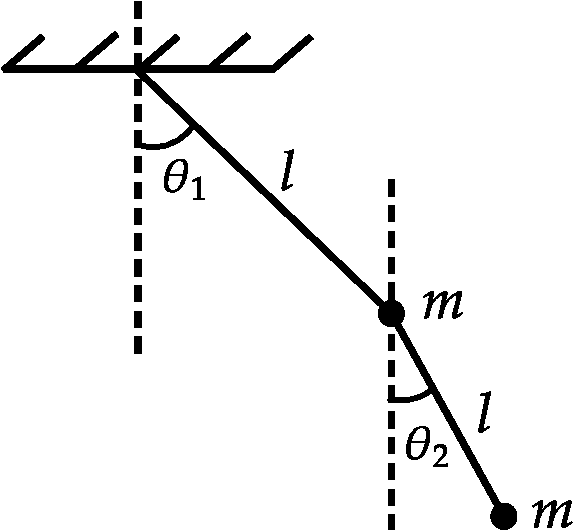
\includegraphics[height=4cm,width=4.5cm]{diagram-20210926(1)-crop}
	\end{figure}
	\begin{tasks}(1)
		\task[\textbf{A.}] $\frac{1}{2} m l^{2}\left[\dot{\theta}_{1}^{2}+\dot{\theta}_{2}^{2}\right]$
		\task[\textbf{B.}] $\frac{1}{2} m l^{2}\left[2 \dot{\theta}_{1}^{2}+\dot{\theta}_{2}^{2}+2 \dot{\theta}_{1} \dot{\theta}_{2} \cos \left(\theta_{1}-\theta_{2}\right)\right]$
		\task[\textbf{C.}] $\frac{1}{2} m l^{2}\left[\dot{\theta}_{1}^{2}+2 \dot{\theta}_{2}^{2}+2 \dot{\theta}_{1} \dot{\theta}_{2} \cos \left(\theta_{1}-\theta_{2}\right)\right]$
		\task[\textbf{D.}] $\frac{1}{2} m l^{2}\left[2 \dot{\theta}_{1}^{2}+\dot{\theta}_{2}^{2}+2 \dot{\theta}_{1} \dot{\theta}_{2} \cos \left(\theta_{1}+\theta_{2}\right)\right]$
	\end{tasks}
	\item A particle of mass $m$ moves inside a bowl. If the surface of the bowl is given by the equation $z=\frac{1}{2} a\left(x^{2}+y^{2}\right)$, where $a$ is a constant, the Lagrangian of the particle is
	{\exyear{NET/JRF(DEC-2011)}}
	\begin{tasks}(2)
		\task[\textbf{A.}] $\frac{1}{2} m\left(\dot{r}^{2}+r^{2} \dot{\phi}^{2}-g a r^{2}\right)$
		\task[\textbf{B.}] $\frac{1}{2} m\left[\left(1+a^{2} r^{2}\right) \dot{r}^{2}+r^{2} \dot{\phi}^{2}\right]$
		\task[\textbf{C.}]  $\frac{1}{2} m\left(\dot{r}^{2}+r^{2} \dot{\theta}^{2}+r^{2} \sin ^{2} \theta \dot{\phi}^{2}-g a r^{2}\right)$
		\task[\textbf{D.}]  $\frac{1}{2} m\left[\left(1+a^{2} r^{2}\right) \dot{r}^{2}+r^{2} \dot{\phi}^{2}-g a r^{2}\right]$
	\end{tasks}
	\item The Lagrangian of a particle of mass $m$ moving in one dimension is given by
	$$
	L=\frac{1}{2} m \dot{x}^{2}-b x
	$$
	where $b$ is a positive constant. The coordinate of the particle $x(t)$ at time $t$ is given by: (in following $c_{1}$ and $c_{2}$ are constants)
	{\exyear{NET/JRF(JUNE-2013)}}
	\begin{tasks}(2)
		\task[\textbf{A.}] $-\frac{b}{2 m} t^{2}+c_{1} t+c_{2}$
		\task[\textbf{B.}] $c_{1} t+c_{2}$
		\task[\textbf{C.}] $c_{1} \cos \left(\frac{b t}{m}\right)+c_{2} \sin \left(\frac{b t}{m}\right)$
		\task[\textbf{D.}] $c_{1} \cosh \left(\frac{b t}{m}\right)+c_{2} \sinh \left(\frac{b t}{m}\right)$
	\end{tasks}	
	\item A particle moves in a potential $V=x^{2}+y^{2}+\frac{z^{2}}{2} .$ Which component(s) of the angular momentum is/are constant(s) of motion?
	{\exyear{NET/JRF(DEC-2013)}}
	\begin{tasks}(4)
		\task[\textbf{A.}] None
		\task[\textbf{B.}] $L_{x}, L_{y}$ and $L_{z}$
		\task[\textbf{C.}]  only $L_{x}$ and $L_{y}$
		\task[\textbf{D.}] only $L_{z}$
	\end{tasks}
	\item A pendulum consists of a ring of mass $M$ and radius $R$ suspended by a massless rigid rod of length $l$ attached to its rim. When the pendulum oscillates in the plane of the ring, the time period of oscillation is
	{\exyear{NET/JRF(DEC-2013)}}
	\begin{tasks}(2)
		\task[\textbf{A.}] $2 \pi \sqrt{\frac{l+R}{g}}$
		\task[\textbf{B.}] $\frac{2 \pi}{\sqrt{g}}\left(l^{2}+R^{2}\right)^{1 / 4}$
		\task[\textbf{C.}] $2 \pi \sqrt{\frac{2 R^{2}+2 R l+l^{2}}{g(R+l)}}$
		\task[\textbf{D.}] $\frac{2 \pi}{\sqrt{g}}\left(2 R^{2}+2 R l+l^{2}\right)^{1 / 4}$
	\end{tasks}	
	\item Consider a particle of mass $m$ attached to two identical springs each of length $l$ and spring constant $k$ (see the figure). The equilibrium configuration is the one where the springs are unstretched. There are no other external forces on the system. If the particle is given a small displacement along the $x$-axis, which of the following describes the equation of motion for small oscillations?
	{\exyear{NET/JRF(DEC-2013)}}
	\begin{figure}[H]
		\centering
		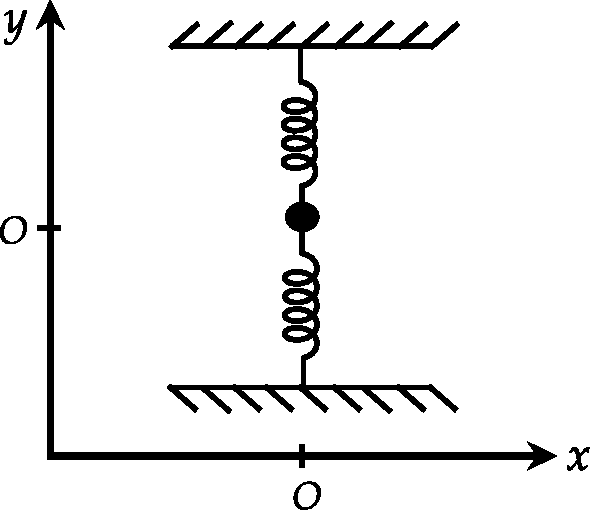
\includegraphics[height=4.5cm,width=5cm]{diagram-20210926(18)-crop}
	\end{figure}
	\begin{tasks}(4)
		\task[\textbf{A.}] $m \ddot{x}+\frac{k x^{3}}{l^{2}}=0$
		\task[\textbf{B.}]  $m \ddot{x}+k x=0$
		\task[\textbf{C.}] $m \ddot{x}+2 k x=0$
		\task[\textbf{D.}] $m \ddot{x}+\frac{k x^{2}}{l}=0$
	\end{tasks}	
	\item The equation of motion of a system described by the time-dependent Lagrangian
	$$
	L=e^{\gamma t}\left[\frac{1}{2} m \dot{x}^{2}-V(x)\right] \text { is }
	$$
	{\exyear{NET/JRF(DEC-2014)}}
	\begin{tasks}(2)
		\task[\textbf{A.}] $m \ddot{x}+\gamma m \dot{x}+\frac{d V}{d x}=0$
		\task[\textbf{B.}] $m \ddot{x}+\gamma m \dot{x}-\frac{d V}{d x}=0$
		\task[\textbf{C.}]  $m \ddot{x}-\gamma m \dot{x}+\frac{d V}{d x}=0$
		\task[\textbf{D.}] $m \ddot{x}+\frac{d V}{d x}=0$
	\end{tasks}
	\item A particle of unit mass moves in the $x y$-plane in such a way that $\dot{x}(t)=y(t)$ and $\dot{y}(t)=-x(t) .$ We can conclude that it is in a conservative force-field which can be derived from the potential
	{\exyear{NET/JRF(JUNE-2015)}}
	\begin{tasks}(4)
		\task[\textbf{A.}] $\frac{1}{2}\left(x^{2}+y^{2}\right)$
		\task[\textbf{B.}] $\frac{1}{2}\left(x^{2}-y^{2}\right)$
		\task[\textbf{C.}] $x+y$
		\task[\textbf{D.}] $x-y$
	\end{tasks}	
	\item The Lagrangian of a particle moving in a plane s given in Cartesian coordinates as
	$$
	L=\dot{x} \dot{y}-x^{2}-y^{2}
	$$
	In polar coordinates the expression for the canonical momentum $p_{r}$ (conjugate to the radial coordinate $r$ ) is
	{\exyear{NET/JRF(DEC-2015)}}
	\begin{tasks}(2)
		\task[\textbf{A.}] $\dot{r} \sin \theta+r \dot{\theta} \cos \theta$
		\task[\textbf{B.}]  $\dot{r} \cos \theta+r \dot{\theta} \sin \theta$
		\task[\textbf{C.}] $2 \dot{r} \cos \theta-r \dot{\theta} \sin 2 \theta$
		\task[\textbf{D.}] $\dot{r} \sin 2 \theta+r \dot{\theta} \cos 2 \theta$
	\end{tasks}
	\item The dynamics of a particle governed by the Lagrangian
	$$
	L=\frac{1}{2} m \dot{x}^{2}-\frac{1}{2} k x^{2}-k x \dot{x} t \text { describes }
	$$
	{\exyear{NET/JRF(DEC-2016)}}
	\begin{tasks}(1)
		\task[\textbf{A.}] An undamped simple harmonic oscillator
		\task[\textbf{B.}] A damped harmonic oscillator with a time varying damping factor
		\task[\textbf{C.}]  An undamped harmonic oscillator with a time dependent frequency
		\task[\textbf{D.}] A free particle
	\end{tasks}	
	\item The parabolic coordinates $(\xi, \eta)$ are related to the Cartesian coordinates $(x, y)$ by $x=\xi \eta$ and $y=\frac{1}{2}\left(\xi^{2}-\eta^{2}\right)$. The Lagrangian of a two-dimensional simple harmonic oscillator of mass $m$ and angular frequency $\omega$ is
	{\exyear{NET/JRF(DEC-2016)}}
	\begin{tasks}(2)
		\task[\textbf{A.}] $\frac{1}{2} m\left[\dot{\xi}^{2}+\dot{\eta}^{2}-\omega^{2}\left(\xi^{2}+\eta^{2}\right)\right]$
		\task[\textbf{B.}] $\frac{1}{2} m\left(\xi^{2}+\eta^{2}\right)\left[\left(\dot{\xi}^{2}+\dot{\eta}^{2}\right)-\frac{1}{4} \omega^{2}\left(\xi^{2}+\eta^{2}\right)\right]$
		\task[\textbf{C.}] $\frac{1}{2} m\left(\xi^{2}+\eta^{2}\right)\left[\dot{\xi}^{2}+\dot{\eta}^{2}-\frac{1}{2} \omega^{2} \xi \eta\right]$
		\task[\textbf{D.}] $\frac{1}{2} m\left(\xi^{2}+\eta^{2}\right)\left[\dot{\xi}^{2}+\dot{\eta}^{2}-\frac{1}{4} \omega^{2}\right]$
	\end{tasks}	
	\item The spring constant $k$ of a spring of mass $m_{s}$ is determined experimentally by loading the spring with mass $M$ and recording the time period $T$, for a single oscillation. If the experiment is carried out for different masses, then the graph that correctly represents the result is
	{\exyear{NET/JRF(DEC-2017)}}
	\begin{tasks}(2)
		\task[\textbf{A.}] \begin{figure}[H]
			\centering
			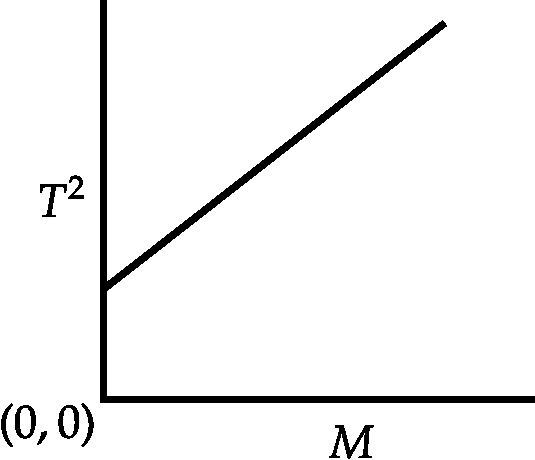
\includegraphics[height=3cm,width=4cm]{diagram-20210926(38)-crop}
		\end{figure}
		\task[\textbf{B.}] \begin{figure}[H]
			\centering
			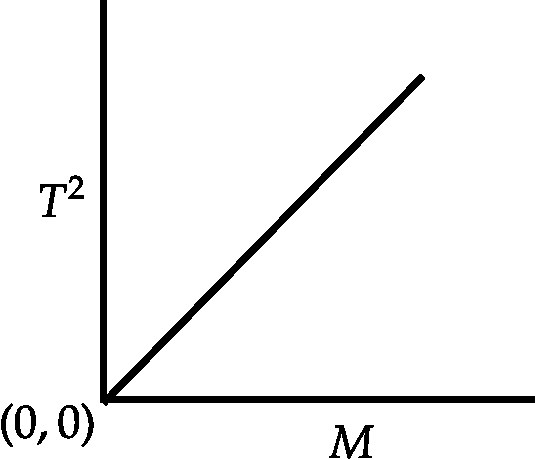
\includegraphics[height=3cm,width=4cm]{diagram-20210926(39)-crop}
		\end{figure}
		\task[\textbf{C.}] \begin{figure}[H]
			\centering
			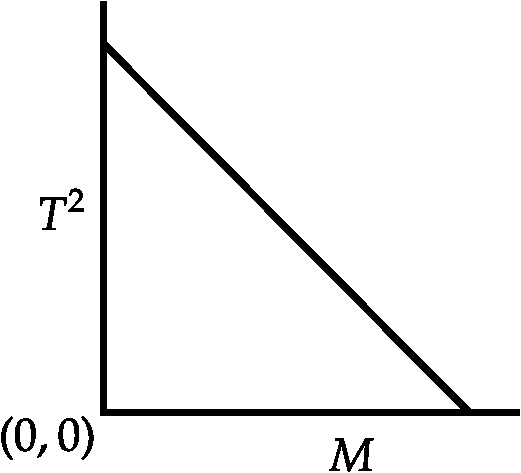
\includegraphics[height=3cm,width=4cm]{diagram-20210926(40)-crop}
		\end{figure}
		\task[\textbf{D.}] \begin{figure}[H]
			\centering
			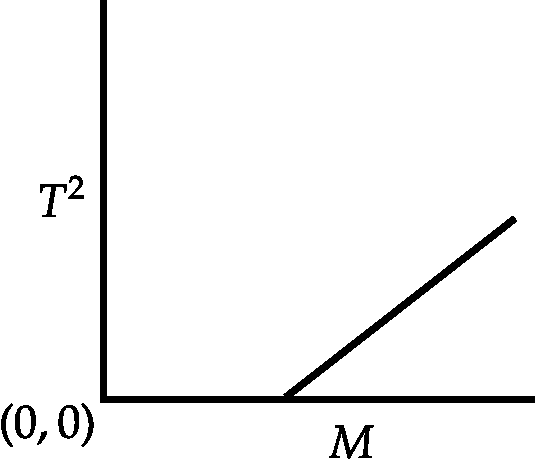
\includegraphics[height=3cm,width=4cm]{diagram-20210926(41)-crop}
		\end{figure}
	\end{tasks}	
	\item The motion of a particle in one dimension is described by the Langrangian $L=\frac{1}{2}\left(\left(\frac{d x}{d t}\right)^{2}-x^{2}\right)$ in suitable units. The value of the action along the classical path from $x=0$ at $t=0$ to $x=x_{0}$ at $t=t_{0}$, is
	{\exyear{NET/JRF(DEC-2018)}}
	\begin{tasks}(4)
		\task[\textbf{A.}] $\frac{x_{0}^{2}}{2 \sin ^{2} t_{0}}$
		\task[\textbf{B.}] $\frac{1}{2} x_{0}^{2} \tan t_{0}$
		\task[\textbf{C.}] $\frac{1}{2} x_{0}^{2} \cot t_{0}$
		\task[\textbf{D.}] $\frac{x_{0}^{2}}{2 \cos ^{2} t_{0}}$
	\end{tasks}	
	\item Two particles of masses $m_{1}$ and $m_{2}$ are connected by a massless thread of length $l$ as shown in figure below.\\
	The particle of mass in on the plane undergoes a circular motion with radius $r_{0}$ and angular momentum $L$. When a small radial displacement $\in$ (whew $\in \ll<r_{0}$ ) is applied, its radial coordinate is found to oscillate about $r_{0}$. The frequency of the oscillations is
	{\exyear{NET/JRF(JUNE-2019)}}
	\begin{tasks}(4)
		\task[\textbf{A.}] $\sqrt{\frac{7 m_{2} g}{\left(m_{1}+\frac{m_{2}}{2}\right) r_{0}}}$
		\task[\textbf{B.}] $\sqrt{\frac{7 m_{2} g}{\left(m_{1}+m_{2}\right) r_{0}}}$
		\task[\textbf{C.}] $\sqrt{\frac{3 m_{2} g}{\left(m_{1}+\frac{m_{2}}{2}\right) r_{0}}}$
		\task[\textbf{D.}] $\sqrt{\frac{3 m_{2} g}{\left(m_{1}+m_{2}\right) r_{0}}}$
	\end{tasks}	
	\item Which of the following terms, when added to the Lagrangian $L(x, y, \dot{x}, \dot{y})$ of a system with two degrees of freedom will not change the equations of motion?\\
	(check question )
	{\exyear{NET/JRF(DEC-2019)}}
	\begin{tasks}(4)
		\task[\textbf{A.}] $x \ddot{x}-y \ddot{y}$
		\task[\textbf{B.}] $x \ddot{y}-y \ddot{x}$
		\task[\textbf{C.}] $x \dot{y}-y \dot{x}$
		\task[\textbf{D.}] $y \dot{x}^{2}+x \dot{y}^{2}$ 
	\end{tasks}
	\item A point mass $m$, is constrained to move on the inner surface of a paraboloid of revolution $x^{2}+y^{2}=a z$ (where $a>0$ is a constant). When it spirals down the surface, under the influence of gravity (along $-z$ direction), the angular speed about the $z$-axis is proportional to
	{\exyear{NET/JRF(JUNE-2020)}}
	\begin{tasks}(2)
		\task[\textbf{A.}] 1 (independent of $z$ )
		\task[\textbf{B.}] $z$
		\task[\textbf{C.}]  $z^{-1}$
		\task[\textbf{D.}] $z^{-2}$
	\end{tasks}	
\end{enumerate}
 \colorlet{ocre1}{ocre!70!}
\colorlet{ocrel}{ocre!30!}
\setlength\arrayrulewidth{1pt}
\begin{table}[H]
	\centering
	\arrayrulecolor{ocre}
	\begin{tabular}{|p{1.5cm}|p{1.5cm}||p{1.5cm}|p{1.5cm}|}
		\hline
		\multicolumn{4}{|c|}{\textbf{Answer key}}\\\hline\hline
		\rowcolor{ocrel}Q.No.&Answer&Q.No.&Answer\\\hline
		1&\textbf{b} &2&\textbf{d}\\\hline 
		3&\textbf{a} &4&\textbf{d} \\\hline
		5&\textbf{c} &6&\textbf{a} \\\hline
		7&\textbf{a}&8&\textbf{a}\\\hline
		9&\textbf{d}&10&\textbf{d}\\\hline
		11&\textbf{b} &12&\textbf{a}\\\hline
		13&\textbf{c}&14&\textbf{d}\\\hline
		15&\textbf{b}&16&\textbf{c}\\\hline
		
	\end{tabular}
\end{table}
\newpage
\begin{abox}
	Practice Set-2
\end{abox}
\begin{enumerate}
	\item A particle of mass $m$ slides under the gravity without friction along the parabolic path $y=a x^{2}$, as shown in the figure. Here $a$ is a constant.\\
	\begin{figure}[H]
		\centering
		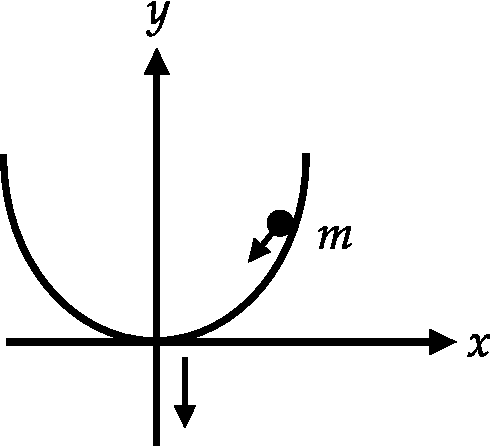
\includegraphics[height=4.5cm,width=5cm]{diagram-20210915(2)-crop}
	\end{figure}
	The Lagrangian for this particle is given by
	{	\exyear{GATE 2012}}
	\begin{tasks}(2)
		\task[\textbf{A.}] $L=\frac{1}{2} m \dot{x}^{2}-m g a x^{2}$
		\task[\textbf{B.}] $L=\frac{1}{2} m\left(1+4 a^{2} x^{2}\right) \dot{x}^{2}-m g a x^{2}$
		\task[\textbf{C.}] $L=\frac{1}{2} m \dot{x}^{2}+m g a x^{2}$
		\task[\textbf{D.}] $L=\frac{1}{2} m\left(1+4 a^{2} x^{2}\right) \dot{x}^{2}+m g a x^{2}$
	\end{tasks}
	\item  The Lagrange's equation of motion of the particle for above question is given by
	{\exyear{GATE 2012}}
	\begin{tasks}(2)
		\task[\textbf{A.}] $\ddot{x}=2 g a x$
		\task[\textbf{B.}] $m\left(1+4 a^{2} x^{2}\right) \ddot{x}=-2 m g a x-4 m a^{2} x \dot{x}^{2}$
		\task[\textbf{C.}] $m\left(1+4 a^{2} x^{2}\right) \ddot{x}=2 m g a x+4 m a^{2} x \dot{x}^{2}$
		\task[\textbf{D.}] $\ddot{x}=-2 g a x$
	\end{tasks}
	\item The Lagrangian of a system with one degree of freedom $q$ is given by $L=\alpha \dot{q}^{2}+\beta q^{2}$, where $\alpha$ and $\beta$ are non-zero constants. If $p_{q}$ denotes the canonical momentum conjugate to $q$ then which one of the following statements is CORRECT?
	{\exyear{GATE 2013}}
	\begin{tasks}(1)
		\task[\textbf{A.}] $p_{q}=2 \beta q$ and it is a conserved quantity.
		\task[\textbf{B.}]  $p_{q}=2 \beta q$ and it is not a conserved quantity.
		\task[\textbf{C.}] $p_{q}=2 \alpha \dot{q}$ and it is a conserved quantity.
		\task[\textbf{D.}]  $p_{q}=2 \alpha \dot{q}$ and it is not a conserved quantity.
	\end{tasks}
	\item A bead of mass $m$ can slide without friction along a massless rod kept at $45^{\circ}$ with the vertical as shown in the figure. The rod is rotating about the vertical axis with a constant angular speed $\omega$. At any instant $r$ is the distance of the bead from the origin. The momentum conjugate to $r$ is
	{\exyear{GATE 2014}}
	\begin{figure}[H]
		\centering
		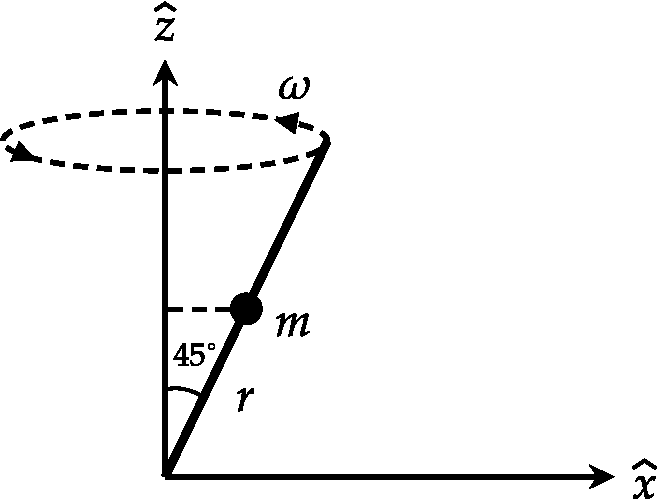
\includegraphics[height=3cm,width=5cm]{diagram-20210915(4)-crop}
	\end{figure}
	\begin{tasks}(4)
		\task[\textbf{A.}] $m \dot{r}$
		\task[\textbf{B.}] $\frac{1}{\sqrt{2}} m \dot{r}$
		\task[\textbf{C.}] $\frac{1}{2} m \dot{r}$
		\task[\textbf{D.}] $\sqrt{2} m \dot{r}$
	\end{tasks}
	\item The Lagrangian of a system is given by
	$L=\frac{1}{2} m l^{2}\left[\dot{\theta}^{2}+\sin ^{2} \theta \dot{\varphi}^{2}\right]-m g l \cos \theta$, where $m, l$ and $g$ are constants.
	Which of the following is conserved?
	{\exyear{GATE 2016}}
	\begin{tasks}(4)
		\task[\textbf{A.}] $\dot{\varphi} \sin ^{2} \theta$
		\task[\textbf{B.}] $\dot{\varphi} \sin \theta$
		\task[\textbf{C.}] $\frac{\dot{\varphi}}{\sin \theta}$
		\task[\textbf{D.}] $\frac{\dot{\varphi}}{\sin ^{2} \theta}$
	\end{tasks}
	\item If the Lagrangian $L_{0}=\frac{1}{2} m\left(\frac{d q}{d t}\right)^{2}-\frac{1}{2} m \omega^{2} q^{2}$ is modified to $L=L_{0}+\alpha q\left(\frac{d q}{d t}\right)$, which one of the following is TRUE?
	{\exyear{GATE 2017}}
	\begin{tasks}(1)
		\task[\textbf{A.}] Both the canonical momentum and equation of motion do not change
		\task[\textbf{B.}] Canonical momentum changes, equation of motion does not change
		\task[\textbf{C.}] Canonical momentum does not change, equation of motion changes
		\task[\textbf{D.}] Both the canonical momentum and equation of motion change
	\end{tasks}
	\item  A double pendulum consists of two equal masses $m$ suspended by two strings of length $l$. What is the Lagrangian of this system for oscillations in a plane? Assume the angles $\theta_{1}, \theta_{2}$ made by the two strings are small (you can use $\cos \theta=1-\theta^{2} / 2$ ).\\
	Note: $\omega_{0}=\sqrt{g / l}$.
	{\exyear{JEST 2014}}
	\begin{tasks}(1)
		\task[\textbf{A.}] $L \approx m l^{2}\left(\dot{\theta}_{1}^{2}+\frac{1}{2} \dot{\theta}_{2}^{2}-\omega_{0}^{2} \theta_{1}^{2}-\frac{1}{2} \omega_{0}^{2} \theta_{2}^{2}\right)$
		\task[\textbf{B.}]  $L \approx m l^{2}\left(\dot{\theta}_{1}^{2}+\frac{1}{2} \dot{\theta}_{2}^{2}+\dot{\theta}_{1} \dot{\theta}_{2}-\omega_{0}^{2} \theta_{1}^{2}-\frac{1}{2} \omega_{0}^{2} \theta_{2}^{2}\right)$
		\task[\textbf{C.}] $L \approx m l^{2}\left(\dot{\theta}_{1}^{2}+\frac{1}{2} \dot{\theta}_{2}^{2}-\dot{\theta}_{1} \dot{\theta}_{2}-\omega_{0}^{2} \theta_{1}^{2}-\frac{1}{2} \omega_{0}^{2} \theta_{2}^{2}\right)$
		\task[\textbf{D.}]  $L \approx m l^{2}\left(\frac{1}{2} \dot{\theta}_{1}^{2}+\frac{1}{2} \dot{\theta}_{2}^{2}+\dot{\theta}_{1} \dot{\theta}_{2}-\omega_{0}^{2} \theta_{1}^{2}-\omega_{0}^{2} \theta_{2}^{2}\right)$
	\end{tasks}
	\item A bike stuntman rides inside a well of frictionless surface given by $z=a\left(x^{2}+y^{2}\right)$, under the action of gravity acting in the negative $z$ direction. $\vec{g}=-g \hat{z} .$ What speed should be maintain to be able to ride at a constant height $z_{0}$ without falling down?
	{\exyear{JEST 2015}}
	\begin{tasks}(1)
		\task[\textbf{A.}] $\sqrt{g z_{0}}$
		\task[\textbf{B.}] $\sqrt{3 g z_{0}}$
		\task[\textbf{C.}] $\sqrt{2 g z_{0}}$
		\task[\textbf{D.}] The biker will not be able to maintain a constant height, irrespective of speed.
	\end{tasks}
	\item The Lagrangian of a particle is given by $L=\dot{q}^{2}-q \dot{q}$. Which of the following statements is true?
	{\exyear{JEST 2015}}
	\begin{tasks}(1)
		\task[\textbf{A.}]  This is a free particle
		\task[\textbf{B.}] The particle is experiencing velocity dependent damping
		\task[\textbf{C.}] The particle is executing simple harmonic motion
		\task[\textbf{D.}] The particle is under constant acceleration.
	\end{tasks}
	\item A hoop of radius a rotates with constant angular velocity $\omega$ about the
	vertical axis as shown in the figure. A bead of mass $m$ can slide on the
	hoop without friction. If $g<\omega^{2} a$ at what angle $\theta$ apart from 0 and $\pi$ is the bead stationary (i.e., $\frac{d \theta}{d t}=\frac{d^{2} \theta}{d t^{2}}=0$ )?
	{\exyear{JEST 2016}}
	\begin{figure}[H]
		\centering
		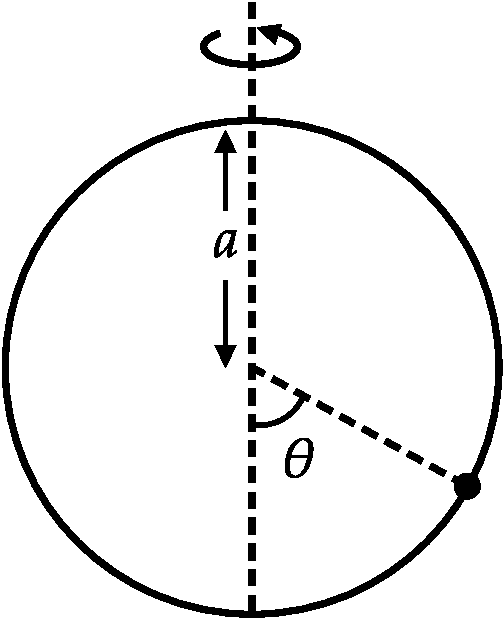
\includegraphics[height=4.2cm,width=3.5cm]{diagram-20210809(11)-crop}
		\caption{}
		\label{}
	\end{figure}
	\begin{tasks}(4)
		\task[\textbf{A.}] $\tan \theta=\frac{\pi g}{\omega^{2} a}$
		\task[\textbf{B.}] $\sin \theta=\frac{g}{\omega^{2} a}$
		\task[\textbf{C.}] $\cos \theta=\frac{g}{\omega^{2} a}$
		\task[\textbf{D.}] $\tan \theta=\frac{g}{\pi \omega^{2} a}$
	\end{tasks}
	\item A bead of mass $M$ slides along a parabolic wire described by $z=2\left(x^{2}+y^{2}\right)$. The wire rotates with angular velocity $\Omega$ about the $z$ - axis. At what value of $\Omega$ does the bead maintain a constant nonzero height under the action of gravity along $-\hat{z}$ ?
	{\exyear{JEST 2017}}
	\begin{tasks}(4)
		\task[\textbf{A.}] $\sqrt{3 g}$
		\task[\textbf{B.}] $\sqrt{g}$
		\task[\textbf{C.}] $\sqrt{2 g}$
		\task[\textbf{D.}] $\sqrt{4 g}$
	\end{tasks}
	\item A possible Lagrangian for a free particle is
	{\exyear{JEST 2017}}
	\begin{tasks}(4)
		\task[\textbf{A.}] $L=\dot{q}^{2}-q^{2}$
		\task[\textbf{B.}] $L=\dot{q}^{2}-q \dot{q}$
		\task[\textbf{C.}] $L=\dot{q}^{2}-q$
		\task[\textbf{D.}] $L=\dot{q}^{2}-\frac{1}{q}$
	\end{tasks}
	\item  A rod of mass $m$ and length $l$ is suspended from two massless vertical springs with a spring constants $k_{1}$ and $k_{2} .$ What is the Lagrangian for the system, if $x_{1}$ and $x_{2}$ be the displacements from equilibrium position of the two ends of the rod?
	{\exyear{JEST 2017}}
	\begin{tasks}(2)
		\task[\textbf{A.}] $\frac{m}{8}\left(\dot{x}_{1}^{2}+2 \dot{x}_{1} \dot{x}_{2}+\dot{x}_{2}^{2}\right)-\frac{1}{2} k_{1} x_{1}^{2}-\frac{1}{2} k_{2} x_{2}^{2}$
		\task[\textbf{B.}] $\frac{m}{2}\left(\dot{x}_{1}^{2}+\dot{x}_{1} \dot{x}_{2}+\dot{x}_{2}^{2}\right)-\frac{1}{4}\left(k_{1}+k_{2}\right)\left(x_{1}^{2}+x_{2}^{2}\right)$
		\task[\textbf{C.}] $\frac{m}{6}\left(\dot{x}_{1}^{2}+x_{1} \dot{x}_{2}+\dot{x}_{2}^{2}\right)-\frac{1}{2} k_{1} x_{1}^{2}-\frac{1}{2} k_{2} x_{2}^{2}$
		\task[\textbf{D.}] $\frac{m}{2}\left(\dot{x}_{1}^{2}-2 \dot{x}_{1} \dot{x}_{2}+\dot{x}_{2}^{2}\right)-\frac{1}{4}\left(k_{1}-k_{2}\right)\left(x_{1}^{2}+x_{2}^{2}\right)$
	\end{tasks}
	\item Consider the Lagrangian
	$$L=1-\sqrt{1-\dot{q}^{2}}-\frac{q^{2}}{2}$$
	of a particle executing oscillations whose amplitude is $A$. If $p$ denotes the momentum of the particle, then $4 p^{2}$ is
	{\exyear{JEST 2015}}
	\begin{tasks}(2)
		\task[\textbf{A.}] (a) $\left(A^{2}-q^{2}\right)\left(4+A^{2}-q^{2}\right)$
		\task[\textbf{B.}] $\left(A^{2}+q^{2}\right)\left(4+A^{2}-q^{2}\right)$
		\task[\textbf{C.}] $\left(A^{2}-q^{2}\right)\left(4+A^{2}+q^{2}\right)$
		\task[\textbf{D.}] $\left(A^{2}+q^{2}\right)\left(4+A^{2}+q^{2}\right)$
	\end{tasks}	
	\item Consider the motion of a particle in two dimensions given by the Lagrangian $$L=\frac{m}{2}\left(\dot{x}^{2}+\dot{y}^{2}\right)-\frac{\lambda}{4}(x+y)^{2}$$
	where $\lambda>0$. The initial conditions are given as $y(0)=0, x(0)=42$ meters, $\dot{x}(0)=\dot{y}(0)=0$. What is the value of $x(t)-y(t)$ at $t=25$ seconds in meters?
	{\exyear{JEST 2019}}
\end{enumerate}
 \colorlet{ocre1}{ocre!70!}
\colorlet{ocrel}{ocre!30!}
\setlength\arrayrulewidth{1pt}
\begin{table}[H]
	\centering
	\arrayrulecolor{ocre}
	\begin{tabular}{|p{1.5cm}|p{1.5cm}||p{1.5cm}|p{1.5cm}|}
		\hline
		\multicolumn{4}{|c|}{\textbf{Answer key}}\\\hline\hline
		\rowcolor{ocrel}Q.No.&Answer&Q.No.&Answer\\\hline
		1&\textbf{b} &2&\textbf{b}\\\hline 
		3&\textbf{d} &4&\textbf{a} \\\hline
		5&\textbf{a} &6&\textbf{b} \\\hline
		7&\textbf{b}&8&\textbf{c}\\\hline
		9&\textbf{a}&10&\textbf{c}\\\hline
		11&\textbf{d} &12&\textbf{b}\\\hline
		13&\textbf{c}&14&\textbf{a}\\\hline
		15&\textbf{42}& &\\\hline
		
	\end{tabular}
\end{table}
\newpage
\begin{abox}
	Practice Set-3
\end{abox}
\begin{enumerate}
	\item A particle of mass $m$ moves inside a bowl under gravity. If the surface of the bowl is given by the equation $z=\frac{1}{2} a\left(x^{2}+y^{2}\right)$, where $a$ is a constant.\\
		(a) Write down Lagrangian of the system in cylindrical coordinate.\\
		(b) Identify the cyclic coordinate and law of conservation of momentum.\\
		(c) Write down the equation of motion
	\begin{answer}
		\begin{align*}
		\text{There is only one particle, so }N&=1\\
		\text{Cartesian coordinate kinetic energy is }T&=\frac{1}{2} m\left(\dot{x}^{2}+\dot{y}^{2}+\dot{z}^{2}\right)\text{ and potential energy is} V=m g z\\
		\text{Equation of Constraint is -}\\
		\text{1. Particle is constrained to move on }&\text{surface of a bowl, so the equation of constraint is}\\
		z&=\frac{1}{2} a\left(x^{2}+y^{2}\right) \text {, so } k=1\\
		\text{Degree of freedom }( DOF) &=3 N-k=3 \times 1-1=2\\
		\text{Hence, there are two degree of  }&\text{ freedom, so we need two generalized coordinates.}\\
		\text{Now transforming the Cartesian coordinate to }&\text{cylindrical coordinate, $x=r \cos \theta, y=r \sin \theta$, z=z}
		\intertext{So, the kinetic energy is $T=\frac{1}{2} m\left(\dot{r}^{2}+r^{2} \dot{\theta}^{2}+\dot{z}^{2}\right)$. And the equation of constraint in cylindrical coordinate $\left(z=\frac{1}{2} a r^{2}\right)$ is written as $\dot{z}=a r \dot{r}$}
		\intertext{So, kinetic energy for two degree of freedom with suitable coordinate is given by, $T=\frac{m}{2}\left(\dot{r}^{2}+r^{2} \dot{\theta}^{2}+a^{2} r^{2} \dot{r}^{2}\right)$ and potential energy $V=\frac{m g a r^{2}}{2}$}
		T=\frac{m}{2}\left(\dot{r}^{2}+r^{2} \dot{\theta}^{2}+a^{2} r^{2} \dot{r}^{2}\right)&\text{ and potential energy }V=\frac{m g a r^{2}}{2}\\
		\text{So, Lagrangian is }L&=\frac{m}{2}\left[\dot{r}^{2}\left(1+a^{2} r^{2}\right)+r^{2} \dot{\theta}^{2}-a g r^{2}\right]
		\intertext{(b) Hence, $\frac{\partial L}{\partial \theta}=0$ so, $\theta$ is cyclic coordinate hence $p_{\theta}=\frac{\partial L}{\partial \dot{\theta}}=m r^{2} \dot{\theta}$ is a constant of motion, which is identified as angular momentum of the system. So angular momentum of the system is conserved.}
		\text{	(c) If Lagrangian of the system is } L&=\frac{m}{2}\left[\dot{r}^{2}\left(1+a^{2} r^{2}\right)+r^{2} \dot{\theta}^{2}-a g r^{2}\right]\text{ then}\\
		\text{Equation of Motion is }&\frac{d}{d t}\left(\frac{\partial L}{\partial \dot{r}}\right)-\frac{\partial L}{\partial r}=0\\
		\left(\frac{\partial L}{\partial r}\right)=m \dot{r}^{2} a^{2} r+m r \dot{\theta}^{2}&-m a g r\text{ and }\left(\frac{\partial L}{\partial \dot{r}}\right)=m \dot{r}\left(1+a^{2} r^{2}\right)\\
		\Rightarrow \frac{d}{d t}\left(\frac{\partial L}{\partial \dot{r}}\right)=m \ddot{r}\left(1+a^{2} r^{2}\right)&+m \dot{r} a^{2} 2 r \dot{r}=m \ddot{r}\left(1+a^{2} r^{2}\right)+2 m a^{2} r \dot{r}^{2}\\
		\frac{d}{d t}\left(\frac{\partial L}{\partial \dot{r}}\right)-\frac{\partial L}{\partial r}=0 \Rightarrow m \ddot{r}\left(1+a^{2} r^{2}\right)&+2 m a^{2} r \dot{r}^{2}-m a^{2} r \dot{r}^{2}-m r \dot{\theta}^{2}+m a g r=0\\
		\Rightarrow m \ddot{r}\left(1+a^{2} r^{2}\right)&+m a^{2} r^{2}-m r \dot{\theta}^{2}+m a g r=0
		\end{align*}
	\end{answer}
	\item A mass $m$ is attached to one end of spring with spring constant $k$ and natural length $l$. The other end is pivoted at point $O$ as shown in figure. If the particle is constrained to move in $x-y$ plane under gravity (in $y$ direction)\\
		(a) Write down the expression for kinetic energy and potential energy.\\
		(b) Write down Lagarngian in Cartesian coordinate system.\\
		(c) Transform the Lagrangian in suitable coordinate system.\\
		\begin{figure}[H]
			\centering
			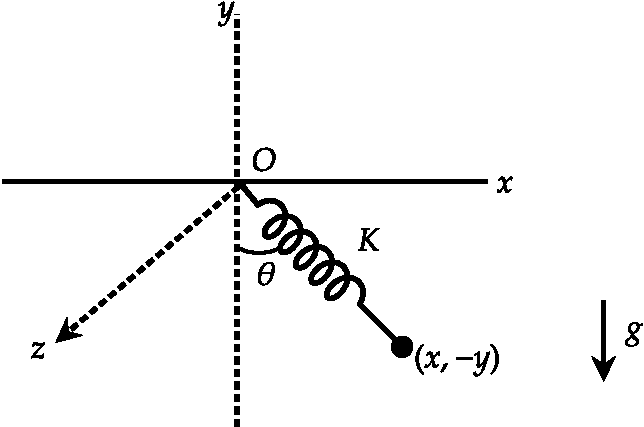
\includegraphics[height=3.8cm,width=5.5cm]{VP-01}
		\end{figure}
	\begin{answer}
		\begin{align*}
		\intertext{ (a) Number of particle $N=1$, kinetic energy is given by $T=\frac{1}{2} m\left(\dot{x}^{2}+\dot{y}^{2}+\dot{z}^{2}\right)$, potential energy is given by $V=-m g y .$}
		\text{Equation of Constraint is -}\\
		\text{The particle is constrained to move in }&x-y\text{ plane so equation of constraint }z=0 \Rightarrow k=1\\
		\text{So, degree of freedom }( \text{ DOF } )&=3 N-K=3 \times 1-1=2\\
		\text{If degree of freedom is two then there}&\text{ must be two independent motion.}\\
		z&=0 \Rightarrow \dot{z}=0
		\intertext{So, $T=\frac{1}{2} m\left(\dot{x}^{2}+\dot{y}^{2}\right)$ and $V=-m g y+\frac{1}{2} k\left[\sqrt{\left(x^{2}+y^{2}\right)}-l\right]^{2}$ (potential energy due to gravity and stored energy due to spring).}
		\text{Lagrangian in the Cartesian coordinate is }L&=\frac{1}{2} m\left(\dot{x}^{2}+\dot{y}^{2}\right)-\left(-m g y+\frac{1}{2} k\left[\sqrt{\left(x^{2}+y^{2}\right)}-l\right]^{2}\right),\\
			L&=\frac{1}{2} m\left(\dot{x}^{2}+\dot{y}^{2}\right)+m g y-\frac{1}{2} k\left[\sqrt{\left(x^{2}+y^{2}\right)}-l\right]^{2}
		\end{align*}
		(b) These two independent motions are in (i) radial direction and (ii) angular direction in plane so best coordinate system to define the system is circular polar coordinate.\\
		But one should express the Lagrangian into suitable coordinate which must be independent of radial and angular variable.
		\begin{align*}
		\text{Put }x&=r \sin \theta, y=r \cos \theta,\text{ so, Lagrangian is given by -}\\
		L&=\frac{1}{2} m\left(\dot{r}^{2}+r^{2} \dot{\theta}^{2}\right)+m g r \cos \theta-\frac{1}{2} k(r-l)^{2}\\
		\text{The equation of }&\text{motion in terms of variable $r$ is }\frac{d}{d t}\left(\frac{\partial L}{\partial \dot{r}}\right)-\frac{\partial L}{\partial r}=0\\
		&\left(\frac{\partial L}{\partial \dot{r}}\right)=m \dot{r} \Rightarrow \frac{d}{d t}\left(\frac{\partial L}{\partial \dot{r}}\right)=m \ddot{r} \text { and }\left(\frac{\partial L}{\partial r}\right)=m r \dot{\theta}^{2}+m g \cos \theta-k(r-l) \\
		&\frac{d}{d t}\left(\frac{\partial L}{\partial \dot{r}}\right)-\frac{\partial L}{\partial r}=0 \Rightarrow m \ddot{r}-m r \dot{\theta}^{2}-m g \cos \theta+k(r-l)=0
		\intertext{The equation of motion in terms of variable $\theta$}
		\left(\frac{\partial L}{\partial \dot{\theta}}\right)&=m r^{2} \dot{\theta}\left(\frac{\partial L}{\partial \theta}\right)=-m g r \sin \theta\\
		\frac{d}{d t}\left(\frac{\partial L}{\partial \dot{\theta}}\right)&=m r^{2} \ddot{\theta}+2 m r \dot{r} \dot{\theta}\\
		\frac{d}{d t}\left(\frac{\partial L}{\partial \dot{\theta}}\right)-\frac{\partial L}{\partial \theta}&=0 \Rightarrow m r^{2} \ddot{\theta}+2 m r \dot{r} \dot{\theta}+m g r \sin \theta=0
		\end{align*}
	\end{answer}
	\item A spherical pendulum of length $a$ moves in a space about fixed point $O$.\\
		(a) Write down Lagrangian of the system.\\
		(b) Identify cyclic Coordinate\\
		(c) Solve Lagrangian equation of motion.\\
		\begin{figure}[H]
			\centering
			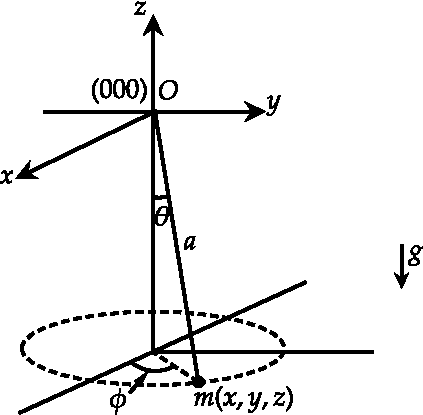
\includegraphics[height=5cm,width=6cm]{VP-02}
		\end{figure}
	\begin{answer}
		\begin{align*}
		\text{Number of particle }N&=1\text{ so }T=\frac{1}{2} m\left(\dot{x}^{2}+\dot{y}^{2}+\dot{z}^{2}\right)\text{ and potential}\\
		\text{energy of system is }V&=-m g z
		\intertext{Equation of Constraint is -}
		\text{(1) The length of pendulum is fixed }&\sqrt{x^{2}+y^{2}+z^{2}}=a\text{ so }K=1\\
		\text{So, degree of freedom }&(\mathrm{DOF})=3 . N-K=3.1-1=2
		\intertext{So there is a need of two generalized coordinates to solve the equation of motion. There are two independent motion (i) angular motion of particle from $z$-axis (ii) angular motion in $x-y$ plane about $z$ axis.}\\
		\text{So, suitable coordinate is spherical }&\text{coordinate.}\\
		x&=r \sin \theta \cos \phi, y=r \sin \theta \sin \phi, z=r \cos \theta\\
		\text{	From equation }&\text{of constraint, }r=a \Rightarrow \dot{r}=0\\
		\text{Kinetic energy }T&=\frac{1}{2} m\left(a^{2} \dot{\theta}^{2}+a^{2} \sin ^{2} \theta \dot{\phi}^{2}\right), \text{potential energy }V=-m g a \cos \theta\\
		L=T-V&=\frac{1}{2} m\left(a^{2} \dot{\theta}^{2}+a^{2} \sin ^{2} \theta \dot{\phi}^{2}\right)+m g a \cos \theta\\
		\text{(b) }\frac{\partial L}{\partial \phi}=0\text{ so }\phi\text{ is cyclic coordinate }\frac{\partial L}{\partial \dot{\phi}}&=p_{\phi}=m a^{2} \sin ^{2} \theta \dot{\phi}\text{ is constant of motion.}\\
		\text{(c) }\frac{d}{d t}\left(\frac{\partial L}{\partial \dot{\theta}}\right)-\left(\frac{\partial L}{\partial \theta}\right)&=0\\
		\left(\frac{\partial L}{\partial \dot{\theta}}\right)=m a^{2} \dot{\theta} \Rightarrow \frac{d}{d t}\left(\frac{\partial L}{\partial \dot{\theta}}\right)&=m a^{2} \ddot{\theta} \Rightarrow\left(\frac{\partial L}{\partial \theta}\right)=m a^{2} \sin \theta \cos \theta \dot{\phi}^{2}-m g a \sin \theta\\
		\text{So, }\frac{d}{d t}\left(\frac{\partial L}{\partial \dot{\theta}}\right)-\left(\frac{\partial L}{\partial \theta}\right)&=0 \Rightarrow m a^{2} \ddot{\theta}-m a^{2} \sin \theta \cos \theta \dot{\phi}^{2}+m g a \sin \theta=0
		\end{align*}
	\end{answer}
	\item A particle of mass $m$ is constrained to move under gravity in inner surface of cone of half angle $\alpha$ as shown in figure.\\
		(a) Write down Lagrangian in suitable coordinate system\\
		(b) Identify cyclic coordinate and discuss conservation of momentum\\
		(c) Write down Lagrange's equation of motion\\
		\begin{figure}[H]
			\centering
			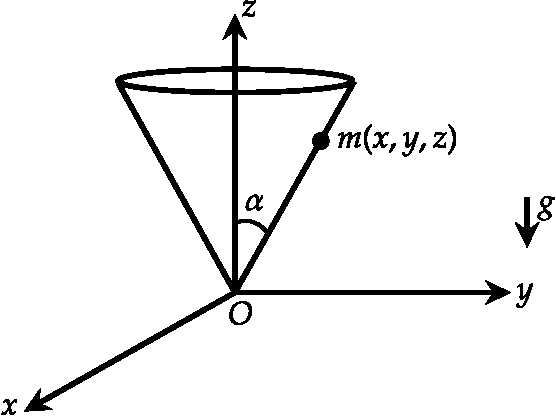
\includegraphics[height=4cm,width=5cm]{VP-03}
		\end{figure}
	\begin{answer}$\left. \right. $\\
		\begin{figure}[H]
			\centering
			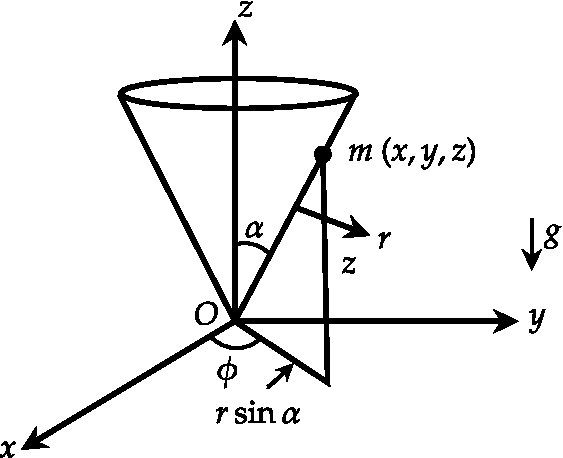
\includegraphics[height=4cm,width=5cm]{VP-04}
		\end{figure}
		\begin{align*}
		\intertext{ A particle of mass $m$ is constrained to move in inner surface of cone of half angle $\alpha$ and $x, y, z$ are the coordinates of particle at any time $t$.}
		&\text{(a) Number of particle $N=1$ so kinetic energy of the system is } T=\frac{1}{2} m\left(\dot{x}^{2}+\dot{y}^{2}+\dot{z}^{2}\right)\\
		&\text{	Assuming that the origin is at the vertex of the cone, the potential energy is given by $V=m g z$}\\
		&\text{ Equation of Constraint is -}\\
		&\text{	Particle is constraint to move on surface of cone where }\tan \alpha=\frac{\sqrt{x^{2}+y^{2}}}{z},\text{ so }K=1.\\
		&\text{So, degree of freedom (DOF) }=3 N-K=3 \times 1-1=2\\
		&\text{So, there is a need of two generalized Coordinates to write the Lagrangian.}
		\end{align*}
		The two independent motion is (i) Linear motion along the slope and (ii) angular motion about $z$ axis. So, spherical symmetry is suitable coordinate.
		\begin{align*}
		\text{Put the value of }x&=r \sin \theta \cos \phi, y=r \sin \theta \sin \phi, z=r \cos \theta\\
		\text{Which gives }T&=\frac{1}{2} m\left(\dot{r}^{2}+r^{2} \dot{\theta}^{2}+r^{2} \sin ^{2} \theta \dot{\phi}^{2}\right)\text{ and }V=m g r \cos \theta\\
		\text{As }\tan \alpha&=\frac{\sqrt{x^{2}+y^{2}}}{z} \Rightarrow \tan \alpha=\tan \theta \Rightarrow \theta=\alpha \Rightarrow \dot{\theta}=0
		\intertext{If Lagrangian of the system is given by $L=\frac{1}{2} m\left(\dot{r}^{2}+r^{2} \sin ^{2} \alpha \dot{\phi}^{2}\right)-m g r \cos \alpha$ there is two generalized coordinates i.e., $r, \phi$}
		\text{(b) }L&=\frac{1}{2} m\left(\dot{r}^{2}+r^{2} \sin ^{2} \alpha \dot{\phi}^{2}\right)-m g r \cos \alpha\\
		\text{One can see Lagrangian }&\text{ not explicitly dependent on $\phi$, which gives $\frac{\partial L}{\partial \phi}=0$. So, $\phi$ is cyclic coordinate.}
		\intertext{$\left(\frac{\partial L}{\partial \dot{\phi}}\right)=p_{\phi} \Rightarrow m r^{2} \sin ^{2} \alpha \dot{\phi}=c$ and $p_{\phi}=c$ so angular momentum of the system is constant during the motion.}
		\intertext{(c) The Lagrangian equation of motion in $r$ variable is given by $\frac{d}{d t}\left(\frac{\partial L}{\partial \dot{r}}\right)-\frac{\partial L}{\partial r}=0$, which gives
			$\left(\frac{\partial L}{\partial \dot{r}}\right)=m \dot{r},\left(\frac{\partial L}{\partial r}\right)=m r \sin ^{2} \alpha \dot{\phi}^{2}-m g \cos \alpha$}
		\intertext{$\frac{d}{d t}\left(\frac{\partial L}{\partial \dot{r}}\right)-\frac{\partial L}{\partial r}=0 \Rightarrow m \ddot{r}-m r \sin ^{2} \alpha \dot{\phi}^{2}+m g \cos \alpha=0$, which is equivalent to Newton's law of motion}
		\end{align*}
	\end{answer}
		\item The system is shown in the figure. The particle $m_{2}$ moves on a vertical axis and the whole system rotates about this axis with a constant angular velocity $\omega$.\\
		(a) Write down Lagrangian of the system in spherical polar co-ordinate.\\
		(b) Discuss conservation of momentum\\
		(c) Write down equation of motion.\\
		\begin{figure}[H]
			\centering
			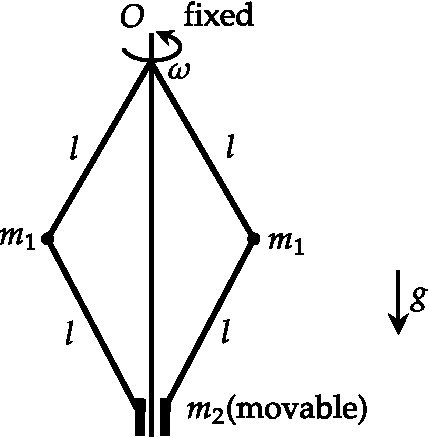
\includegraphics[height=4.2cm,width=4.3cm]{VP-05}
		\end{figure}
	\begin{answer}$\left. \right. $\\
		\begin{figure}[H]
			\centering
			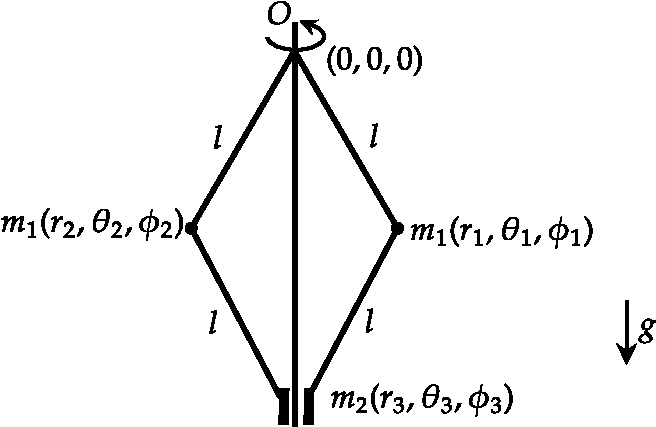
\includegraphics[height=4.1cm,width=6.5cm]{VP-06}
		\end{figure}
		\begin{align*}
		\text{(a) Number of }&\text{Particle,} N=3\\
		\text{The kinetic}&\text{ energy  is given by}\\
		T&=\frac{1}{2} m_{1}\left(\dot{x}_{1}^{2}+\dot{y}_{1}^{2}+\dot{z}_{1}^{2}\right)+\frac{1}{2} m_{2}\left(\dot{x}_{2}^{2}+\dot{y}_{2}^{2}+\dot{z}_{2}^{2}\right)+\frac{1}{2} m_{3}\left(\dot{x}_{3}^{2}+\dot{y}_{3}^{2}+\dot{z}_{3}^{2}\right)\\
		\text{Potential  }&\text{energy assuming $O$ as origin}\\
		V&=-m_{1} g z_{1}-m_{1} g z_{2}-m_{2} g z_{3}\\
		x_{1}&=r_{1} \sin \theta_{1} \cos \phi_{1}, y_{1}=r_{1} \sin \theta_{1} \sin \phi_{1}, z_{1}=r_{1} \cos \theta_{1}\\
		x_{2}&=r_{2} \sin \theta_{2} \cos \phi_{2}, y_{2}=r_{2} \sin \theta_{2} \sin \phi_{2}, z_{2}=r_{2} \cos \theta_{2}\\
		x_{3}&=r_{3} \sin \theta_{3} \cos \phi_{3}, y_{3}=r_{3} \sin \theta_{3} \sin \phi_{3}, z_{3}=r_{3} \cos \theta_{3}\\
		\text{The kinetic  }&\text{energy in spherical coordinate is given by}\\
		T&=\frac{1}{2} m_{1}\left(\dot{r}_{1}^{2}+r_{1}^{2} \dot{\theta}_{1}^{2}+r_{1}^{2} \sin ^{2} \theta_{1}^{2} \dot{\phi}_{1}^{2}\right)+\frac{1}{2} m_{2}\left(\dot{r}_{2}^{2}+r_{2}^{2} \dot{\theta}_{2}^{2}+r_{2}^{2} \sin ^{2} \theta_{2}^{2} \dot{\phi}_{2}^{2}\right)\\
		&+\frac{1}{2} m_{3}\left(\dot{r}_{3}^{2}+r_{3}^{2} \dot{\theta}_{3}^{2}+r_{3}^{2} \sin ^{2} \theta_{3}^{2} \dot{\phi}_{3}^{2}\right)\\
		\text{And potential }&\text{energy is given by }V=-m_{1} g r_{1} \cos \theta_{1}-m_{2} g r_{2} \cos \theta_{2}-m_{3} g r_{3} \cos \theta_{3}\\
		\text{Equations of }&\text{Constraint are -}
		\end{align*}
		\begin{enumerate}
		\item  Length of mass $m_{1}$ from origin $O$ is fixed, $r_{1}=l$
		\item  Length of another mass $m_{2}$ from origin $O$ is fixed, $r_{2}=l$
		\item  Both masses $m_{1}$ and $m_{2}$ make same angle with $z$ - axis, $\theta_{1}=\theta_{2}=\theta$
		\item  Both masses $m_{1}$ make angle in the $x-y$ plane with $x$ axis as $\phi_{1}=\phi_{2}+c$
		\item  Particle $m_{2}$ makes angle zero with $z$ - axis i.e., $\theta_{3}=0$
		\item  Particle $m_{2}$ makes angle zero in $x-y$ plane with $x$ axis i.e., $\phi_{3}=0$,\\
		\item  Particle $m_{2}$ have distance $r_{3}=2 l \cos \theta$ from origin $O$.
		So, $K=7$.\\ So degree of freedom (DOF) $=3 N-K=3\times 3-7=2$\\
		There is two independent motion.\\
		(i.) linear motion of $m_{2}$ on $z$ axis and (ii) both mass $m_{1}$ rotating about $z$ axis. So there is a need of two generalized coordinates. Using equation of constraint one will transform Lagrangian as $L=T-V$
		\end{enumerate}
		\begin{align*}
		L&=m_{1} l^{2}\left(\dot{\theta}^{2}+\dot{\phi}^{2} \sin ^{2} \theta\right)+2 m_{2} l^{2} \dot{\theta}^{2} \sin ^{2} \theta+2\left(m_{1}+m_{2}\right) g l \cos \theta\\
		\text{	Put the value of }\dot{\phi}&=\omega,\text{ then Lagrangian is given by}\\
		L&=m_{1} l^{2}\left(\dot{\theta}^{2}+\omega^{2} \sin ^{2} \theta\right)+2 m_{2} l^{2} \dot{\theta}^{2} \sin ^{2} \theta+2\left(m_{1}+m_{2}\right) g l \cos \theta\\
		\text{(b) }\left(\frac{\partial L}{\partial \phi}\right)&=0\text{ so $\phi$ is cyclic coordinate hence conjugate momentum}\\ \left(\frac{\partial L}{\partial \dot{\phi}}\right)&=\left(\frac{\partial L}{\partial \omega}\right)=p_{\phi}=2 m_{1} l^{2} \omega \sin ^{2} \theta\\
		\text{is constant during  }&\text{the motion. So, $z$ - component of angular momentum is conserved.}\\
		\text{(c) }&\frac{d}{d t}\left(\frac{\partial L}{\partial \dot{\theta}}\right)-\frac{\partial L}{\partial \theta}=0\\
		&\left(\frac{\partial L}{\partial \dot{\theta}}\right)=\left(2 m_{1} l^{2} \dot{\theta}+4 m_{2} l^{2} \dot{\theta} \sin ^{2} \theta\right) \\
		&\frac{d}{d t}\left(\frac{\partial L}{\partial \dot{\theta}}\right)=\left(2 m_{1} l^{2}+4 m_{2} l^{2} \sin ^{2} \theta\right) \ddot{\theta}+4 m_{2} l^{2} \sin 2 \theta \dot{\theta}^{2} \\
		&\left(\frac{\partial L}{\partial \theta}\right)=m_{1} l^{2} \omega^{2} 2 \sin \theta \cos \theta+2 m_{2} l^{2} \dot{\theta}^{2} 2 \sin \theta \cos \theta-2\left(m_{1}+m_{2}\right) g l \sin \theta\\
		\text{The equation }&\text{of  motion is given as -}\\
		\frac{d}{d t}\left(\frac{\partial L}{\partial \dot{\theta}}\right)&-\frac{\partial L}{\partial \theta}=0\\
		\left(2 m_{1} l^{2}+4 m_{2} l^{2} \sin ^{2} \theta\right) \ddot{\theta}&+2 m_{2} l^{2} \sin 2 \theta \dot{\theta}^{2}-m_{1} l^{2} \omega^{2} \sin 2 \theta+2\left(m_{1}+m_{2}\right) g l \sin \theta=0
		\end{align*}
	\end{answer}
	\item 
		If kinetic energy and potential energy is given by $T=\frac{1}{2} m\left(\dot{x}^{2}+\dot{y}^{2}\right)$ and $V=-m g y$ respectively.
		\begin{tasks}(1)
			\task[\textbf{a.}] Write down Lagrangian of the system.
			\task[\textbf{b.}] Identify generalized coordinate and generalized velocity.
			\task[\textbf{c.}] Identify cyclic coordinate and discuss conservation of momentum.
			\task[\textbf{d.}]  Discuss equation of motion.
		\end{tasks}
	\begin{answer}
		\begin{align*}
		\text{(a)}\quad L=T-V \Rightarrow \frac{1}{2} m\left(\dot{x}^{2}+\dot{y}^{2}\right)&-(-m g y) \Rightarrow \frac{1}{2} m\left(\dot{x}^{2}+\dot{y}^{2}\right)+m g y\\
		\text{(b)}\quad \text{ Generalized coordinate }q_{1}&=x, q_{2}=y\text{ generalized velocity} \dot{q}_{1}=\dot{x}, \dot{q}_{2}=\dot{y}\\
		\text{(c)} \quad\left(\frac{\partial L}{\partial q_{1}}\right)&=\left(\frac{\partial L}{\partial x}\right)=0, \text{so it is a cyclic coordinate}\\ 
		\text{Then} \left(\frac{\partial L}{\partial \dot{x}}\right)&=p_{x}=m \dot{x}, \\
		\text{Identified as linear momentum }&\text{in $x$ direction is constant of motion.}\\
		\left(\frac{\partial L}{\partial y}\right)&=m g \neq 0,\text{ so it is not cyclic coordinate}\\
		\text{(d)} \quad\frac{d}{d t}\left(\frac{\partial L}{\partial \dot{x}}\right)-\left(\frac{\partial L}{\partial x}\right)&=0 \\ 
		\frac{d}{d t} m \dot{x}-0&=0 \Rightarrow m \dot{x}=c,\\
		 \text{which is exactly explained in}&\text{ section (b)} \\
		\frac{d}{d t}\left(\frac{\partial L}{\partial \dot{y}}\right)-\left(\frac{\partial L}{\partial y}\right)&=0 \\ \frac{d}{d t} m \dot{y}-m g&=0 \Rightarrow m \ddot{y}-m g=0
		\end{align*}
	\end{answer}
	\item 
		Atwood's machine \\
		\begin{figure}[H]
			\centering
			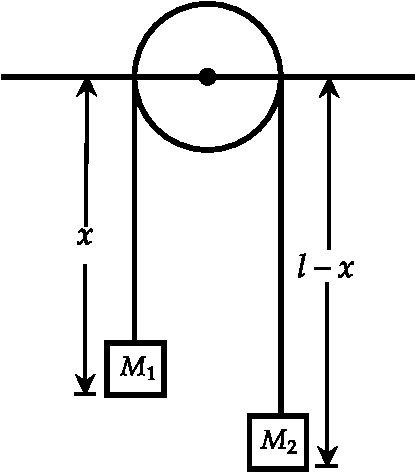
\includegraphics[height=4.7cm,width=4cm]{EP-04}
		\end{figure}
	\begin{answer}
		\begin{align*}
		\intertext{A conservative system with holonomic, scleronomous constraint  (the pulley is assumed frictionless and massless). There is only one independent coordinate $x$, the position of the other weight being determined by the constraint that the length of the rope between them is $l$. The potential energy is}
		V&=-M_{1} g x-M_{2} g(l-x)\\
		\text{while the kinetic}&\text{  energy is}\\
		T&=\frac{1}{2}\left(M_{1}+M_{2}\right) \dot{x}^{2}\\
		\text{Lagrangian has }&\text{the form}\\
		L&=T-V=\frac{1}{2}\left(M_{1}+M_{2}\right) \dot{x}^{2}+M_{1} g x+M_{2} g(l-x)\\
		\text{equation of}&\text{ motion}\\
		\frac{\partial L}{\partial  x}&=\left(M_{1}-M_{2}\right) g\\
		\frac{\partial  L}{\partial  x}&=\left(M_{1}+M_{2}\right) \dot{x}\\
		\text{$\mathrm{so }$}
		\left(M_{1}+M_{2}\right) \ddot{x}&=\left(M_{1}-M_{2}\right) g,\\
		\ddot{x}&=\frac{M_{1}-M_{2}}{M_{1}+M_{2}} g,\\
		\end{align*}
	\end{answer}
	
	
	
\end{enumerate}